\themaD
\graphicspath{{../../S16_Proportionnalite/Images/}}

\chapter{Proportionnalité}
\label{S16}


%%%%%%%%%%%%%%%%%%%%%%%%%%%%%%
%%%%%%%%%%%%%%%%%%%%%%%%%%%%%%
\begin{autoeval}
   \small
   \begin{enumerate}
      \item Il reconnaît une situation de proportionnalité ou de non-proportionnalité entre deux grandeurs.
      \item Il résout des problèmes de proportionnalité dans diverses situations pouvant faire intervenir des pourcentages ou des échelles. Pour cela, il met en œuvre des procédures variées (additivité, homogénéité, passage à l’unité, coefficient de proportionnalité).
   \end{enumerate}
\end{autoeval}

\begin{prerequis}
   \begin{itemize}
     \item Coefficient de proportionnalité.
     \item[\com] Reconnaître une situation de proportionnalité ou de non-proportionnalité.
     \item[\com] Résoudre des problèmes utilisant la proportionnalité (pourcentages, échelles, agrandissement réduction).
   \end{itemize}
\end{prerequis}

\vfill

\begin{debat}[Défi : ces affreux pourcentages !] 
   La notion de {\bf pourcentage} est très importante dans la vie courante mais c'est un concept relativement mal compris ou mal utilisé, et on trouve régulièrement des erreurs dans les médias. Ces deux vidéos montrent des exemples de pourcentages erronés dans des journaux d'information. \\
   \begin{center}
      \textcolor{B1}{\fontsize{70}{80}\selectfont \%}
   \end{center}
   \bigskip
   \begin{cadre}[B2][J4]
      \begin{center}
         Vidéos : \href{https://www.yout-ube.com/watch?v=ibWzdm_05zs}{\bf Consommation d'huile de palme} et \href{https://www.youtube.com/watch?v=gLbsxj8mv-U}{\bf Facture d'électricité}, issues de journaux télévisés.
      \end{center}
   \end{cadre}
\end{debat}


%%%%%%%%%%%%%%%%%%%%%%%%%%%%%%%%
%%%%%%%%%%%%%%%%%%%%%%%%%%%%%%%%
\activites

\begin{activite}[Le puzzle de Brousseau]
   {\bf Objectifs :} mettre en \oe uvre un ou des moyens pour résoudre un problème d'agrandissement ; reproduire une figure géométrique en respectant des mesures ; rendre compte d'un travail en groupe.
   \begin{QCM}
      \partie[présentation du puzzle]
      Ci-dessous se trouve un puzzle composé de quatre pièces A, B, C et D dont les mesures sont indiquées sur la figure. \\
      \begin{center}
         \begin{pspicture}(-1,-1)(12,11.5)
            \psframe(0,0)(11,11)
            \psline(4,0)(4,9)(11,2)
            \psline(6,11)(0,5)
            \psline[linestyle=dashed,linecolor=gray](11,9)(4,9)
            \rput(2,9){\bf\large A}
            \rput(8.5,7.5){\bf\large B}
            \rput(2,4){\bf\large C}
            \rput(7,3){\bf\large D}
            \rput{90}(11.5,6.5){\ucm{9}}
            \rput{90}(11.5,1){\ucm{2}}
            \rput(8.5,11.5){\ucm{5}}
            \rput(3,11.5){\ucm{6}}
            \rput{90}(-0.5,8){\ucm{6}}
            \rput{90}(-0.5,2.5){\ucm{5}}
            \rput(2,-0.5){\ucm{4}}
            \rput(7.5,-0.5){\ucm{7}}
            \rput{90}(3.5,4){\ucm{9}}
            \rput(8,9.5){\ucm{7}}
         \end{pspicture}
      \end{center}
      \partie[travail demandé]
         Par groupes, vous allez devoir refaire le même puzzle mais en plus grand : il faudra s'accorder sur la procédure à adopter pour agrandir les éléments du puzzle, se répartir la construction des pièces en faisant les calculs individuellement puis assembler les morceaux pour reconstituer le puzzle agrandi. \\
         Le compte-rendu de vos recherches sera présenté sous la forme d’une affiche par groupe.
         \begin{center}
            {\bf C'est parti\dots{} le segment de 4 cm devra mesurer 5 cm sur votre puzzle agrandi.}
         \end{center}
         \bigskip
   \end{QCM}
\end{activite}


%%%%%%%%%%%%%%%%%%%%%%%%%%%%%%
%%%%%%%%%%%%%%%%%%%%%%%%%%%%%%
\cours 

%%%%%%%%%%%%%%%%%%%%%%%%%
\section{Procédures de proportionnalité (rappels)}

\begin{center}
   \begin{pspicture}(0,3.2)(16,8.5)
      \psframe*[fillstyle=solid,linecolor=A3](1.5,7)(8,8.6)
      \rput(4.75,7.8){\parbox{6cm}{\centering {\bf Linéarité additive} \\ 12 stylos = 4 stylos + 4 stylos + 4 stylos \\ coûtent \ueuro{10} +\ueuro{10} + \ueuro{10} = \ueuro{30}}}
      \psframe*[fillstyle=solid,linecolor=A3](9,7)(13.5,8.6)
      \rput(11.25,7.8){\parbox{4cm}{\centering {\bf Linéarité multiplicative} \\ 12 stylos = 3$\times$4 stylos \\ coûtent $3\times\ueuro{10} =\ueuro{30}$}}
      \psframe*[fillstyle=solid,linecolor=A3!50](1.5,2.5)(7,5.1)
      \rput(4.25,3.8){\parbox{5cm}{\centering {\bf Passage par l'unité} \\ 1 stylo coûte 4 fois moins cher : \\ $\ueuro{10}\div4 =\ueuro{2,5}$ \\ 12 stylos coûtent 12 fois plus cher : \\ $12\times\ueuro{2,5} =\ueuro{30}$}}
      \psframe*[fillstyle=solid,linecolor=A3!50](9,2.5)(15.5,5.1)
      \rput(12.25,3.8){\parbox{6cm}{\centering {\bf Coefficient de proportionnalité} \\ $4\times\fbox{2,5} =10$ \\ le coefficient de proportionnalité vaut 2,5 \\ $12\times\fbox{2,5} =30$ \\ 12 stylos coûtent \ueuro{30}}}
      \psellipse[fillstyle=solid,fillcolor=B3](8,6)(2.7,1)
      \rput(8,6){\parbox{4.5cm}{\centering \bf Si 4 stylos coûtent 10 \ueuro{} \\ combien coûtent 12 stylos ?}}
   \end{pspicture}
\end{center}

%%%%%%%%%%%%%%%%%%%%%%%%%%%
\section{Reconnaître une situation de proportionnalité}

Pour reconnaître des grandeurs proportionnelles, on peut vérifier qu'il existe un coefficient de proportionnalité entre elles.
\vspace*{-5mm}

\begin{exemple}
\ \\ [-10mm]
   \begin{itemize}
      \item Le périmètre d'un cercle est-il proportionnel à son rayon ?
      \item L'aire d'un disque est-elle proportionnelle à son rayon ?
   \end{itemize}
   \correction
    \ \\ [-10mm]
       \begin{itemize}
         \item $p =$\fbox{$2\times\pi$}$\times r$. Le coefficient $2\times\pi$ est constant, le périmètre est donc proportionnel à son rayon.
         \item  $A =\pi\times r^2 =$\fbox{$\pi\times r$}$\times r$. La variable $\pi\times r$ varie en fonction de $r$, l'aire n'est donc pas proportionnelle à son rayon.
      \end{itemize}
  \end{exemple}

%%%%%%%%%%%%%%%%
\section{Pourcentages, échelles}

\begin{definition}
   Le {\bf pourcentage} d'une quantité est le nombre qui aurait été proportionnellement obtenu si la quantité avait été de 100.
\end{definition}

\begin{exemple}
   Une promotion sur un jus de fruits indique que la contenance est de 1 L + 20\,\%. \\
      Quelle est la nouvelle contenance ?
   \correction
      Calcul de l'augmentation : $\dfrac{20}{100}\times\ul{1} =\ul{0,2}$. \\
      Calcul de la nouvelle contenance : \\
      $\ul{1}+\ul{0,2} =\ul{1,2}$.
\end{exemple}

\medskip

\begin{definition}
   L'\textbf{échelle} d'une carte est le coefficient de proportionnalité entre la mesure réelle et sa mesure sur la carte, ces deux mesures étant exprimées dans la même unité.
\end{definition}

\begin{exemple*1}
   Une carte au 1/2\,000 signifie que \ucm{1} sur la carte représente \ucm{2000} en réalité, soit \um{20}. On note aussi 1:2 000. \\ [-2mm]
      \Propor[GrandeurA=Distance sur la carte en \ucm{},GrandeurB=Distance dans la réalité en \ukm{}]{1/20,2/40,10/200}
      \FlechesPD{1}{2}{$\times20$}
      \vspace*{-4mm}
\end{exemple*1}


%%%%%%%%%%%%%%%%%%%%%%%%%%%%%%
%%%%%%%%%%%%%%%%%%%%%%%%%%%%%%
\exercicesbase

\begin{colonne*exercice}

\begin{exercice} %1
   Ces situations sont-elles proportionnelles ? \\
   Justifier par un contre-exemple ou une preuve.
   \begin{enumerate}
      \item Taille en mètre en fonction de l'âge ?
      \item Périmètre du carré en fonction de son côté ?
      \item Aire du carré en fonction de son côté ?
      \item Distance parcourue à vélo à vitesse constante en fonction du temps.
   \end{enumerate}
\end{exercice}

\begin{corrige}
   \ \\ [-5mm]
   \begin{enumerate}
      \item Taille en mètre en fonction de l'âge : {\blue non}. \\
         Par exemple, si un enfant mesure \ucm{75} à 1 an, il ne mesurera pas $\ucm{750} =\um{7,5}$ à 10 ans.
      \item Périmètre du carré en fonction de son côté : {\blue oui}. \\
         $\mathcal{P} =4\times c$, 4 étant une constante.
      \item Aire du carré en fonction de son côté  : {\blue non}. \\
         Par exemple, un carré de côté \ucm{1} a une aire de \ucmq{1} et un carré de côté \ucm{2} a une aire de \ucmq{4}.
      \item Distance parcourue à vitesse constante : {\blue oui}. \\
         $d =v\times t$, la vitesse étant constante.
   \end{enumerate}
\end{corrige}

\bigskip


\begin{exercice} %2
   Compléter les tableaux de proportionnalité suivants du prix d'un objet selon la quantité. \\ [-3mm]
   \Propor[GrandeurA=Objets,GrandeurB=Prix (\ueuro{}),Math,Stretch=1.5,Largeur=7mm,CouleurTab=Cornsilk]{1/,12/,8/24,/75}
   \FlechesPD{1}{2}{$\times\dots$}
   \FlechesPG{2}{1}{$\times\dots$} \\ [-8mm]
   \Propor[GrandeurA=Objets,GrandeurB=Prix (\ueuro{}),Math,Stretch=1.5,Largeur=7mm,CouleurTab=Cornsilk]{/3,/10,/26,60/}
   \FlechesPD{1}{2}{$\div5$}
   \FlechesPG{2}{1}{$\times\dots$}
\end{exercice}

\begin{corrige}
\ \\ [-10mm]
   \Propor[GrandeurA=Objets,GrandeurB=Prix (\ueuro{}),Math,Stretch=1.5,Largeur=7mm,CouleurTab=Cornsilk]{1/\textcolor{blue}{3},12/\textcolor{blue}{36},8/24,\textcolor{blue}{25}/75}
   \FlechesPD{1}{2}{\blue $\times3$}
   \FlechesPG{2}{1}{\blue $\times\frac13$} \\ [-10mm]
   \Propor[GrandeurA=Objets,GrandeurB=Prix (\ueuro{}),Math,Stretch=1.5,Largeur=7mm,CouleurTab=Cornsilk]{\textcolor{blue}{15}/3,\textcolor{blue}{50}/10,\textcolor{blue}{130}/26,60/\textcolor{blue}{12}}
   \FlechesPD{1}{2}{$\div5$}
   \FlechesPG{2}{1}{\blue $\times5$}
\end{corrige}

\bigskip


\begin{exercice} %3
   Rayan a pesé ses beignets et a trouvé que deux beignets pèsent \ug{300} et trois beignets pèsent \ug{450}.
   \begin{enumerate}
      \item Combien pèsent cinq beignets ?
      \item Combien pèsent six beignets ?
      \item Combien pèsent quatorze beignets ?
   \end{enumerate}
\end{exercice}

\begin{corrige}
   \ \\ [-5mm]\begin{enumerate}
      \item 5 beignets $=$ 2 beignets $+$ 3 beignets. \\
         Or, $\ug{300}+\ug{450} =\ug{750}$. \\
         Donc, {\blue 5 beignets pèsent \ug{750}}.
      \item 6 beignets $=2\times3$ beignets.
         Or, $2\times\ug{450} = \ug{900}$. \\
         Donc, {\blue 6 beignets pèsent \ug{900}}.
      \item 14 beignets $=7\times2$ beignets. \\
         Or, $7\times\ug{300} =\ug{2100}$. \\
         Donc, {\blue 14 beignets pèsent \ug{2100}}.
   \end{enumerate}
\end{corrige}

\bigskip


\begin{exercice} %4
   Un robinet qui fuit laisse échapper de façon continue trois litres d’eau en deux heures.
   \begin{enumerate}
      \item Quelle quantité d’eau se sera écoulée au bout d’une demi-journée ?
      \item Quel temps s’est écoulé pour laisser s’échapper \ul{51} ?
      \item L’eau est facturée \ueuro{0,0031} le litre. \\
         Quel sera le montant de la facture au bout d’un an ?
   \end{enumerate}
\end{exercice}

\begin{corrige}
   \ \\ [-5mm]
   \begin{enumerate}
      \item Une demi-journée dure \uh{12}, c'est-à-dire $6\times\uh{2}$. \\
         La quantité d'eau écoulée sera de $6\times\ul{3} =\blue \ul{18}$.
      \item $\ul{51} =17\times\ul{3}$. \\
         Il s'est donc écoulé $17\times\uh{2} =\blue \uh{34}$.
      \item Un an, c'est 365 jours, soit 730 demi-journées. \\
         Il s'écoulera donc $730\times\ul{18} =\ul{13140}$ en un an. \\
         À 0,0031\euro{} le litre, cela fait $13140\times0,0031\text{\euro} \approx\blue \ueuro{41}$.
   \end{enumerate}
\end{corrige}

\bigskip


\begin{exercice} %5
   Au collège de Ginan, le foyer prend en charge 25\,\% du prix des voyages scolaires alors que dans celui de Ludovico, le foyer donne \ueuro{54} pour un voyage de \ueuro{180} et l'aide est proportionnelle au coût du voyage.
   \begin{enumerate}
      \item Si Ginan participe à un voyage qui coûte \ueuro{230}, quel montant est pris en charge par son foyer ?
      \item En proportion, dans quel collège le foyer participe-t-il le plus au financement des voyages ?
   \end{enumerate}
\end{exercice}

\begin{corrige}
   \ \\ [-5mm]
   \begin{enumerate}
      \item $\dfrac{25}{100}\times\ueuro{230} =\ueuro{57,5}$. \\ [2mm]
         Sur \ueuro{230}, {\blue \ueuro{57,5} sont pris en charge par le foyer}.
      \item Au collège de Ginan, le pourcentage pris en charge est de $\dfrac{\ueuro{54}}{\ueuro{180}}\times100 =30\%$. \\ [2mm]
      C'est au {\blue collège de Ginan que la proportion prise en charge par le foyer est la plus élevée}.
   \end{enumerate}
\end{corrige}

\bigskip


\begin{exercice} %6
   Selene fait pour ses amis deux verres contenant des boissons au sirop.
      \begin{enumerate}
         \item Le premier verre a une contenance de \ucl{20} et il y a 3,5\,\% de sirop. Combien cela fait-il de sirop ?
         \item Le deuxième verre contient \ucl{10} de boisson dont 5\,\% de sirop. Combien cela fait-il de sirop ?
         \item Sachant qu'au départ, il y avait \uml{15} de sirop, combien lui reste-t-il de sirop après ces deux verres ?
      \end{enumerate}
\end{exercice}
   
\begin{corrige}
\ \\ [-5mm]
   \begin{enumerate}
      \item 1\up{er} verre : $\dfrac{3,5}{100}\times\ucl{20} =\ucl{0,7}$. \\ [1mm]
         {\blue Le premier verre contient \ucl{0,7} de sirop}. \smallskip
      \item 2\up{e} verre : $\dfrac{5}{100}\times\ucl{10} =\ucl{0,5}$. \\ [1mm]
         {\blue Le deuxième verre contient \ucl{0,7} de sirop}.
      \item Dans les verres, il y a $\ucl{0,7}+\ucl{0,5} =\ucl{1,2}$ de sirop. \\
         Au départ, Selene avait $\uml{15} = \ucl{1,5}$, {\blue il lui restera donc \ucl{0,3} de sirop}.
   \end{enumerate}
\end{corrige}

\bigskip


\begin{exercice} %7
   Reproduire sur le cahier la cocotte à l'échelle 1:2 puis à l'échelle 2:1.
   \begin{center}
      \psset{unit=0.5}
      \begin{pspicture}(8,8)
         \psgrid[subgriddiv=1,linestyle=solid,gridlabels=0,gridcolor=lightgray](0,0)(8,8)
         \psset{linewidth=0.5mm}
         \pspolygon(1,1)(4,1)(5.5,2.5)(7,1)(7,4)(5.5,5.5)(7,7)(4,7)(4,4)
      \end{pspicture}
   \end{center} 
\end{exercice}

\begin{corrige}
   Echelle $1:2$. {\blue On divise les mesures par 2}. \\
   {\psset{unit=0.5}
      \begin{pspicture}(-5,-0.5)(5,5.5)
         \psgrid[subgriddiv=1,linestyle=solid,gridlabels=0,gridcolor=lightgray](0,0)(5,5)
      \psset{unit=0.5}
         \psset{linewidth=0.5mm}
         \pspolygon(2,2)(5,2)(6.5,3.5)(8,2)(8,5)(6.5,6.5)(8,8)(5,8)(5,5)         
      \end{pspicture}} \\
   Echelle $2:1$. {\blue On multiplie les mesures par 2}.
    {\psset{unit=0.5}
        \begin{pspicture}(0,-0.5)(13,14.5)
         \psgrid[subgriddiv=1,linestyle=solid,gridlabels=0,gridcolor=lightgray](0,0)(14,14)
         \psset{linewidth=0.5mm}
         \pspolygon(1,1)(7,1)(10,4)(13,1)(13,7)(10,10)(13,13)(7,13)(7,7)
      \end{pspicture}}
\end{corrige}

\bigskip


\begin{exercice} %8
   D’après le relevé à la main levée du géomètre ci-dessous, tracer le dessin de ce terrain ainsi que la construction qu’il comporte à l’échelle 1:500.
   \begin{center}
      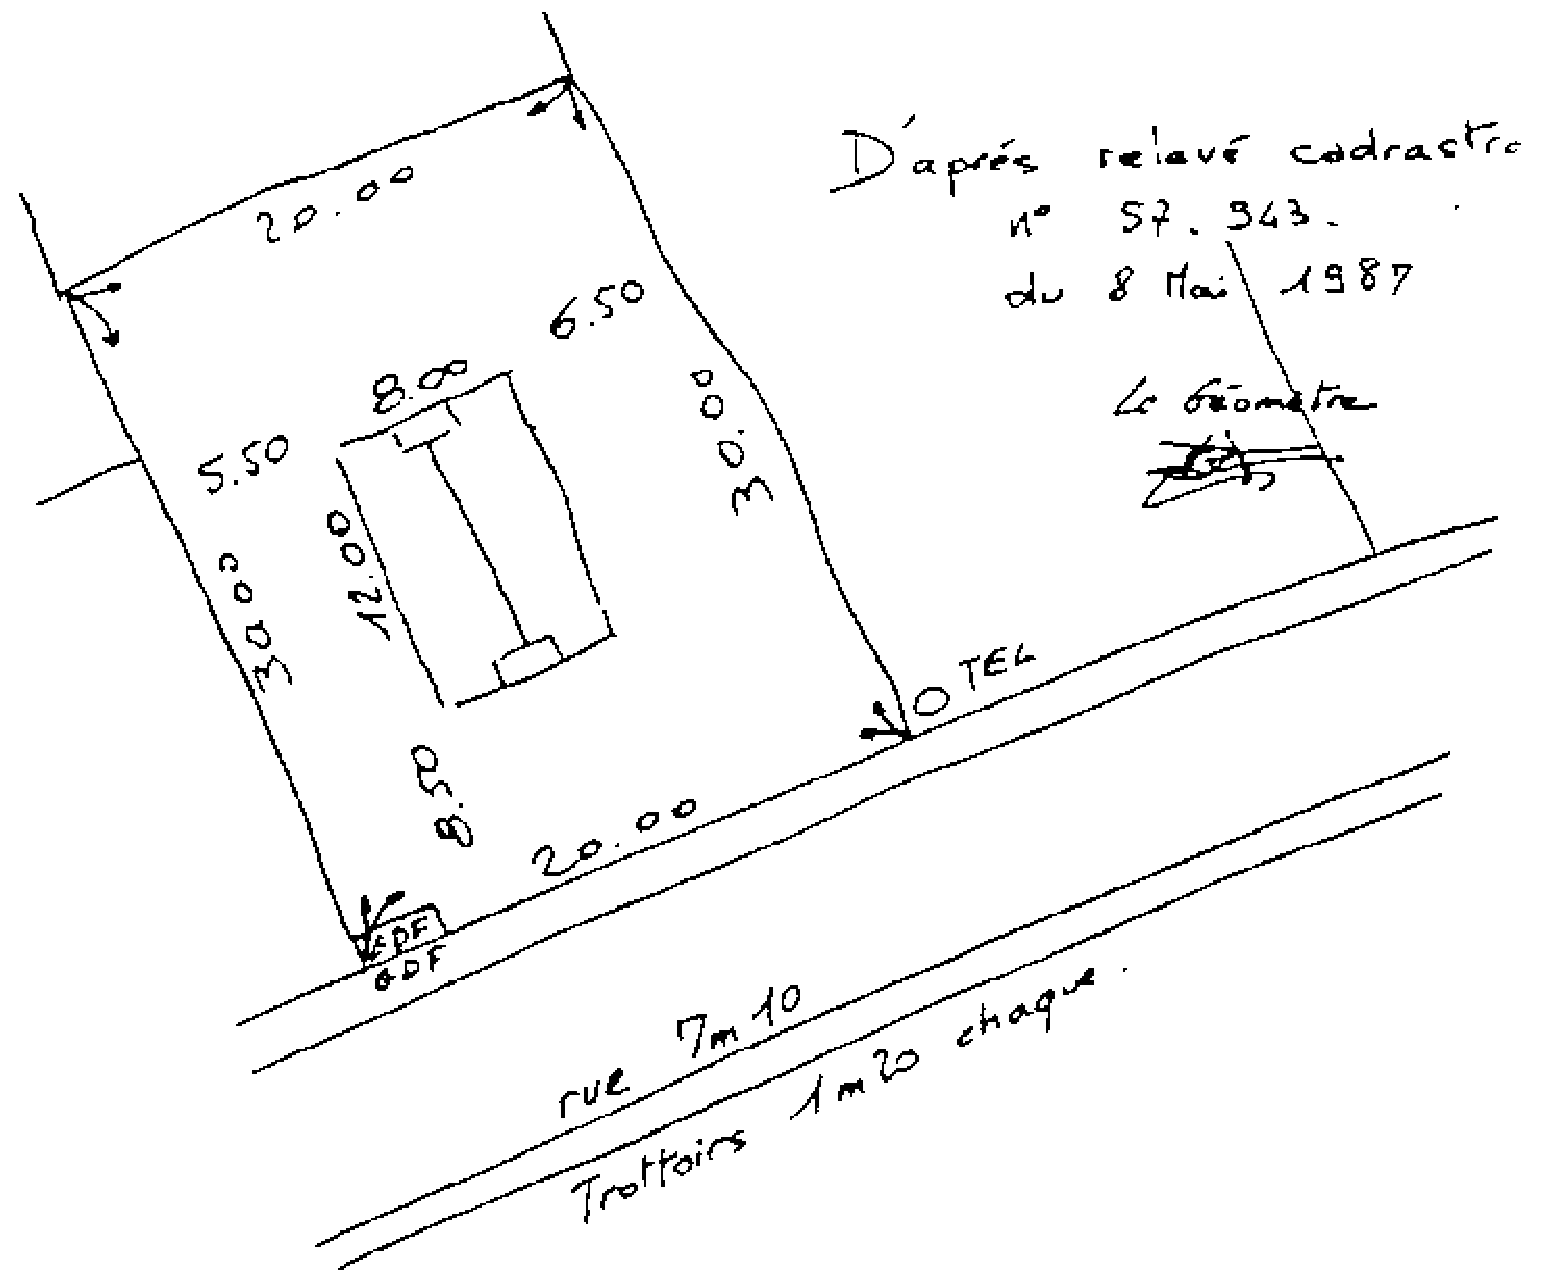
\includegraphics[width=8cm]{cadastre}
   \end{center}
\end{exercice}

\begin{corrige}
   Une échelle au 1:500 signifie que 1 cm sur le dessin représente 500 cm dans la réalité, ou encore 5 m. \\
   Il suffit donc de diviser toutes les dimensions du plan (exprimées en mètre) par 5 pour obtenir les dimensions sur le dessin (exprimées en centimètre). On obtient le dessin ci-dessous : \\
   \begin{center}
      \begin{pspicture}(-1,-1)(5,7)
         \footnotesize
         \psgrid[subgriddiv=2,gridlabels=0pt,gridcolor=lightgray](-1,-1)(5,7)
         \psframe(0,0)(4,6)
         \rput(2,0.25){4 cm}
         \rput{90}(3.75,3){6 cm}
         \rput{90}(0.8,2.8){2,4 cm}
         \rput{90}(1.1,0.8){1,7 cm}
         \rput(1.9,4.35){1,6 cm}
         \rput(0.5,4.1){1,1 cm}
         \rput(3.4,4.1){1,3 cm}
         \psframe(1.1,1.7)(2.7,4.1)
         \psline(-1,0)(5,0)
         \psline(-1,-0.24)(5,-0.24)
      \end{pspicture}
   \end{center}
\end{corrige}

\bigskip


\begin{exercice} %7
   Trois poules pondent dix \oe ufs en deux heures.
   \begin{enumerate}
      \item Combien de poules faudrait-il pour pondre cinq \oe ufs en vingt minutes ?
      \item Combien de temps mettraient neuf poules pour pondre vingt \oe ufs ?
   \end{enumerate}
\end{exercice}

\begin{corrige}
   3 poules pondent 10 \oe ufs en \uh{2} donc : \\
   \begin{enumerate}
      \item 3 poules pondent 5 \oe ufs en $\uh{1} =\umin{60}$ ; \\
         donc, {\blue 9 poules pondent 5 \oe ufs en \umin{20}} (il faut 3 fois plus de poules pour 3 fois moins de temps). \\
      \item 9 poules pondent 5 \oe ufs en \umin{20} ; \\
         donc, {\blue 9 poules pondent 20 \oe ufs en \umin{80}} (il y a 4 fois plus d'\oe ufs, il faut 4 fois plus de temps). \\ [5cm]
   \end{enumerate}
\end{corrige}

\end{colonne*exercice}


%%%%%%%%%%%%%%%%%%%%%%%%%
%%%%%%%%%%%%%%%%%%%%%%%%%
\Recreation

\smallskip

\begin{enigme}[Empreinte carbone]
   \partie[une infographie]
     Voici un extrait d’un document paru dans le quotidien {\it Le Monde} (infographie d’Hélène Pasquier), élaboré à partir de l’Ademe, et intitulé \og Rapport des inégalités du monde 2022 \fg, d’après le ministère de la transition écologique et le Haut conseil pour le climat. \\ [1mm] 
   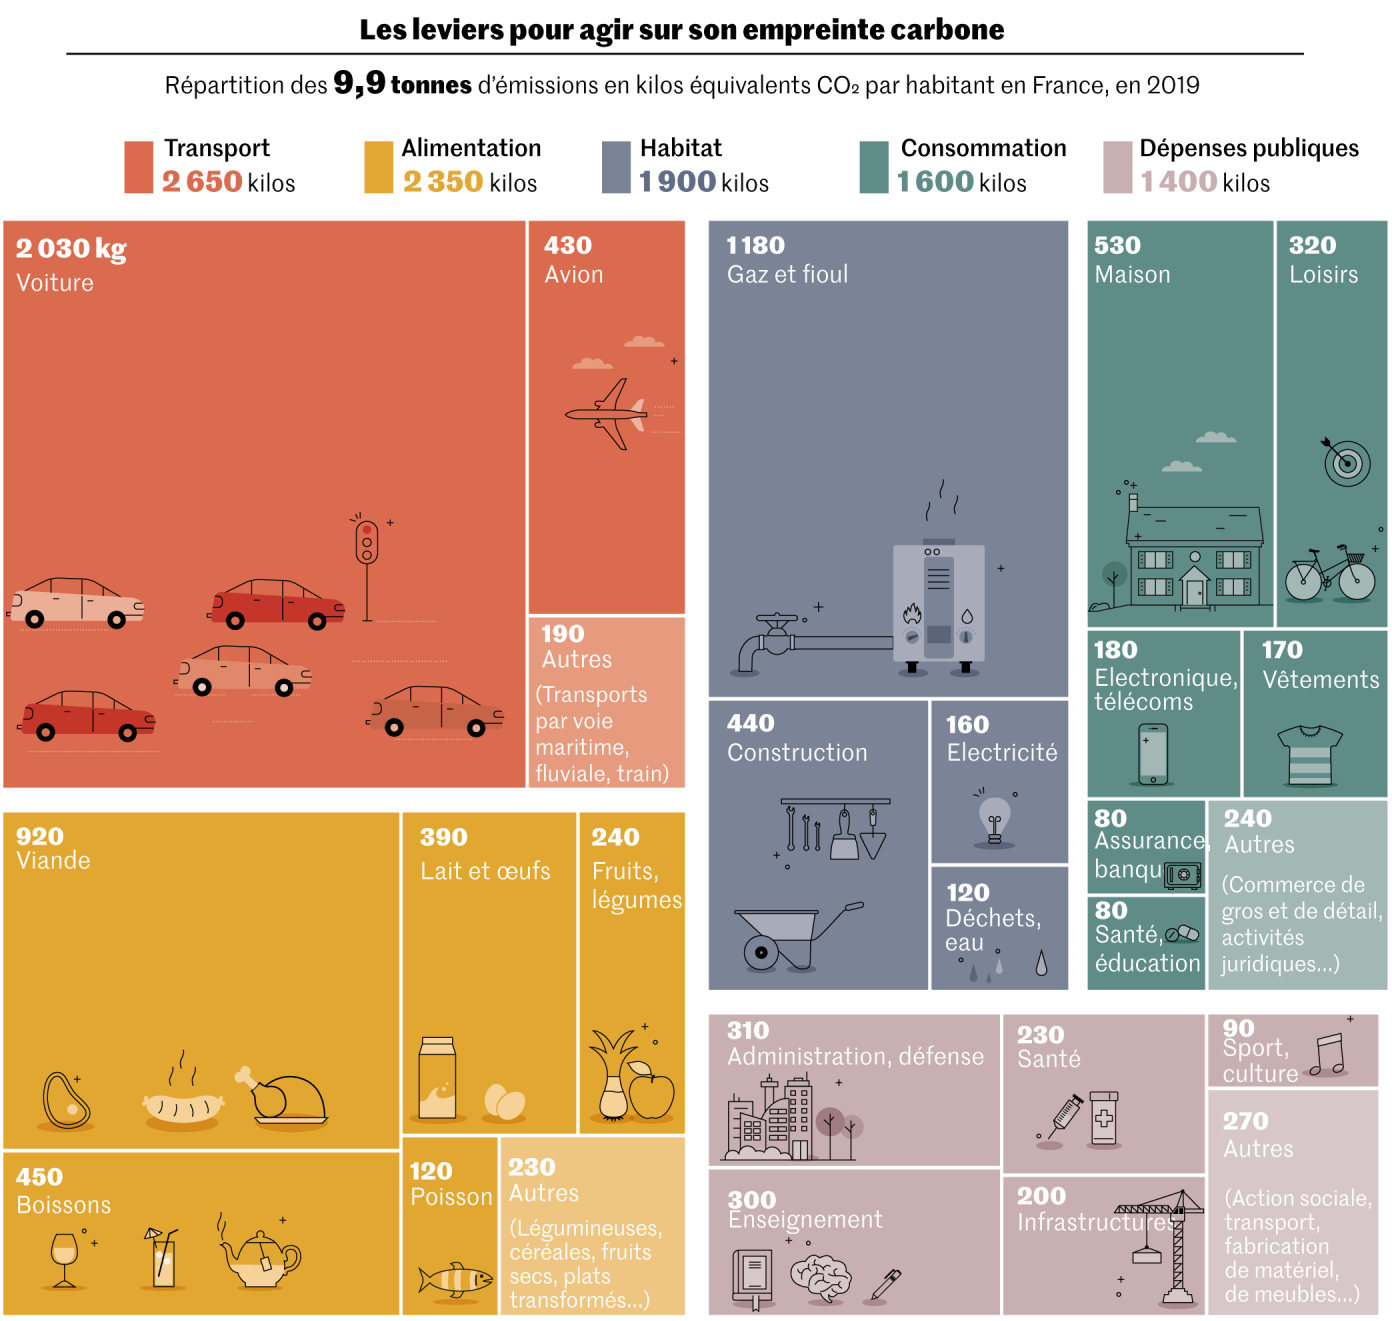
\includegraphics[width=17cm]{carbone} \\ [-3mm]
   
   \partie[la tâche proposée]
      En groupe, trouver une méthode pour vérifier si cette infographie est bien réalisée, en expliquant la méthode. Récapituler les recherches sur une affiche.
\end{enigme}

\vfill\hfill {\it\small Source : d'après une idée de Claire Lommé sur son site \href{https://clairelommeblog.wordpress.com/category/maths-et-societe}{Pierre carrée.}}

\begin{corrige}
   Pour voir si cette infographie est bien réalisée, il faut vérifier que l'aire de chaque \og bulle \fg{} rectangulaire est proportionnelle au nombre de kilos équivalents CO$_{2}$ émis. \smallskip
   
   {\bf 1) On peut commencer par vérifier globalement, par domaine}. \\
   Dans un tableau, on récapitule les données dont on a besoin : longueur de la bulle, hauteur de la bulle, ce qui nous permet de déterminer son aire. Ensuite, on vérifie qu'il y a proportionnalité entre l'aire et l'émission de CO$_{2}$ en calculant, par exemple, le rapport entre les deux. \medskip
   
   {\hautab{1.5}
   \small
   \begin{LCtableau}{\linewidth}{6}{p{2cm}}
      \hline
      & long. & haut. & aire & carb. & rapp. \\
      \hline
      Transport & 8,3 & 6,9 & 57,27 & 2650 & 46,3 \\
      \hline
      Alimentation & 8,3 & 6,1 & 50,63 & 2350 & 46,4 \\
      \hline
      Habitat & 4,4 & 9,4 & 41,36 & 1900 & 45,9 \\
      \hline
      Consommation & 3,6 & 9,4 & 33,84 & 1600 & 47,3 \\
      \hline
      Dépenses pub. & 8,1 & 3,2 & 25,92 & 1400 & 46,7 \\
      \hline
   \end{LCtableau}}
   
   Les rapports sont situés autour de 46-47, on peut donc en déduire que les bulles de domaines sont bien proportionnées (les différences sont dues aux approximations de lecture des grandeurs). \smallskip
   
   {\bf 2) On peut ensuite par vérifier si, par domaine, les bulles détails sont bien réalisées}. \\
   On crée le même type de tableau, par exemple pour le domaine des transports : \medskip
   
   {\hautab{1.5}
   \small
   \begin{LCtableau}{\linewidth}{6}{p{2cm}}
      \hline
      & long. & haut. & aire & carb. & rapp. \\
      \hline
      Voiture & 6,3 & 6,9 & 43,47 & 2030 & 46,7 \\
      \hline
      Avion & 1,9 & 4,8 & 9,12 & 430 & 47,1 \\
      \hline
      Autres & 1,9 & 2,1 & 3,99 & 190 & 47,6 \\
      \hline
   \end{LCtableau}}
   
   Les rapports sont situés autour de 47 également, on peut donc en déduire que les bulles de détails sont bien proportionnées. \smallskip
   
   {\blue En conclusion, on peut légitimement émettre l'hypothèse que le reste de l'infographie est construire sous le même modèle, et donc que cette infographie a les bonnes proportions}.

\end{corrige}


